
   \documentclass{standalone}
   \usepackage{tikz}
   %\usetikzlibrary{positioning,shapes}
   \usepackage{pgfplots}
   \begin{document}
   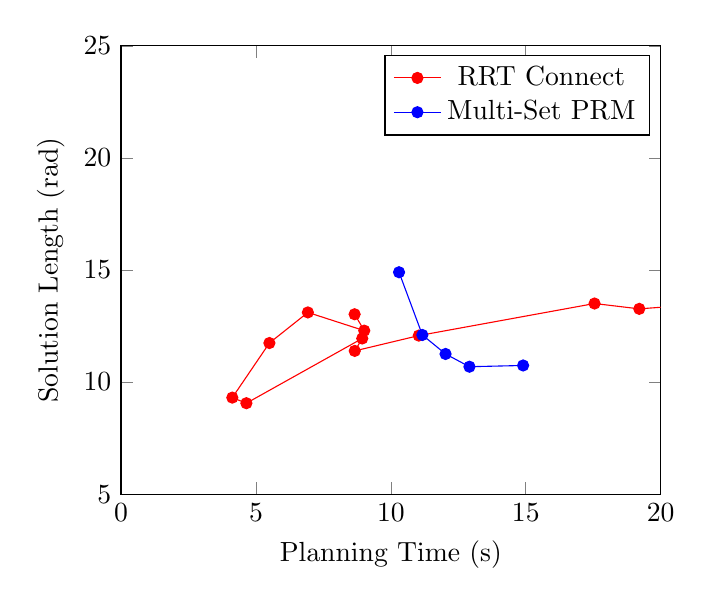
\begin{tikzpicture}
   
   \begin{axis}[
      xlabel=Planning Time (s),
      ylabel=Solution Length (rad),
      ylabel near ticks,
      xlabel near ticks,
      xmin=0,xmax=20,
      ymin=5,ymax=25]
   
   \addplot[mark=*,red] plot coordinates {
     (95.3653789758,15.360278006)
  (40.7783598423,13.7978283385)
  (29.7412340164,14.2061849268)
  (19.2073494196,13.2648273704)
  (17.5494935751,13.5032369187)
  (11.0343671083,12.0722279664)
  (8.66263229848,11.3894957331)
  (8.93958041668,11.9442676519)
  (4.64595172405,9.05621833563)
  (4.12519505024,9.30576064613)
  (5.49895987511,11.7408237521)
  (6.9248734951,13.1061933269)
  (9.01477019787,12.2927640648)
  (8.65738089085,13.0246120223)

   };
   \addlegendentry{RRT Connect}
   
   \addplot[mark=*,blue] plot coordinates {
     (14.9025934935,10.7397690483)
  (12.9133094311,10.6839891368)
  (12.0273448229,11.2527718077)
  (11.1682682037,12.0997075179)
  (10.3035849333,14.8986589073)

   };
   \addlegendentry{Multi-Set PRM}
   
   \end{axis}
   
   \end{tikzpicture}
   \end{document}
   
